\subsubsection {Sauvegarder une partie}
Si vous souhaitez sauvegarder votre partie afin de la reprendre plus tard, allez dans le menu \emph{Fichier} -> \emph{Sauvegarde...}.
Une fenêtre apparaîtra alors pour vous demander de spécifier l'emplacement du fichier de sauvegarde.
Si vous ne souhaitez pas prendre la peine de spécifier cet emplacement, vous pouvez aller dans \emph{Fichier} -> \emph{Sauvegarde rapide}.
Prenez note que cela écrasera votre sauvegarde rapide précédente.

\begin{figure}[!h]
\centering
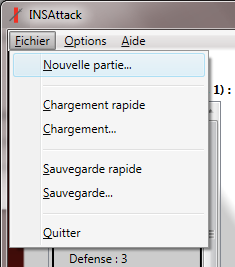
\includegraphics{Parties/Images/Menu.png}
\caption{La menu du jeu}
\label{fig:menu}
\end{figure}

\subsubsection {Charger une partie}
Si vous souhaitez reprendre une partie sauvegardée, allez dans le menu \emph{Fichier} -> \emph{Chargement...}.
Une fenêtre apparaîtra alors pour vous demander de spécifier l'emplacement du fichier à charger.
Il est également possible de charger une partie depuis la fenêtre d'accueil.
Pour charger une partie sauvegardée avec l'option \emph{Sauvegarde rapide}, allez dans \emph{Fichier} -> \emph{Chargement rapide}.

